\section{Polimerizzazione supramolecolare}
\subsection{Polimeri supramolecolari}\begin{frame}\frametitle{Polimeri supramolecolari}
          \vspace{-5pt}  \begin{columns}
\column{0.6\linewidth}   \begin{definition}
              {\bf Supramolecular polymers} are defined as polymeric arrays of monomeric units that are {\bf brought together by reversible and highly directional secondary interactions}, resulting in polymeric properties in dilute and concentrated solution as well as in the bulk. \cite{12}
              \end{definition}\column{0.5\linewidth}
Le interazioni secondarie possono essere:
 \begin{itemize}
  \item legami ad idrogeno;
  \item interazioni di stacking $\pi-\pi$;
  \item interazioni idrofobiche;
  \item legami metallo-legante.
 \end{itemize}\end{columns}\vspace{10pt}
La polimerizzazione è un equilibrio, dunque \textbf{tutto è sotto controllo termodinamico}. Il grado di polimerizzazione del polimero non è stabile a variazioni di temperatura e concentrazione.
\end{frame}




\logo{}

\subsection{Meccanismi di polimerizzazione}\begin{frame}\frametitle{Meccanismi di polimerizzazione}
 \begin{columns}
\column{0.6\linewidth}\begin{itemize}
                       \item Pol. \textbf{isodesmica}: formazione di legami indipendentemente dal polimero, simile a pol. a stadi, alte polidispersità.
                       \item Pol. anello-catena: a basse conc. più anelli, ad alte conc. più catene.
                       \item Pol. \textbf{cooperativa}.
                       \end{itemize}
\column{0.5\linewidth}\vspace{-15pt}\begin{figure}{\centering{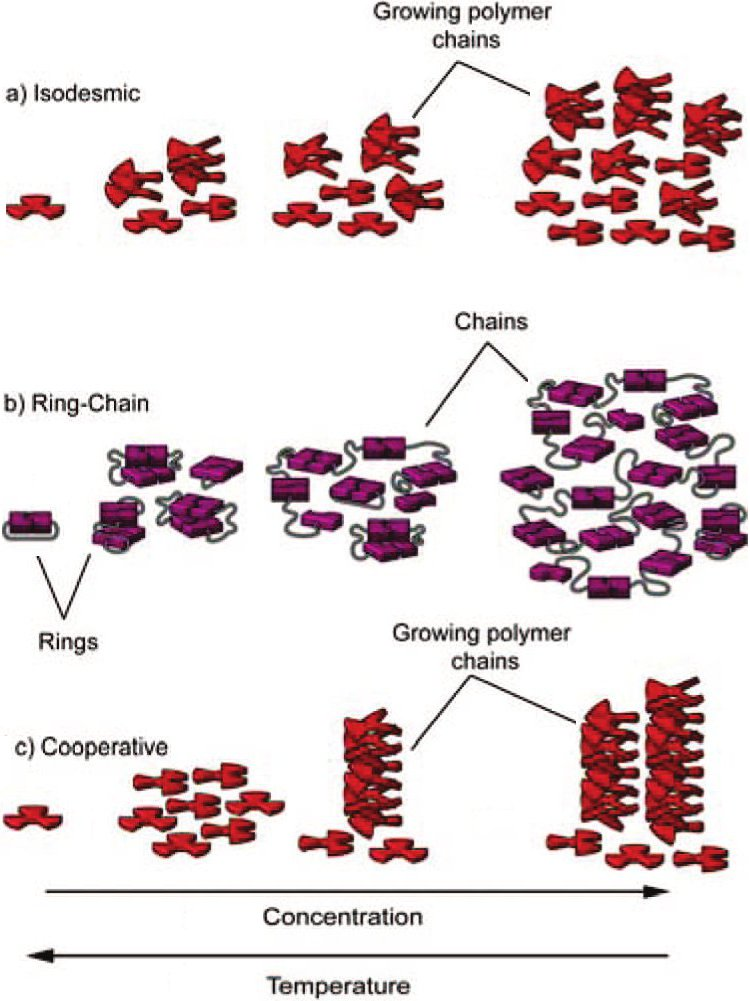
\includegraphics[width=1\textwidth]{sec0/polimerizzazione.jpg}}}\end{figure}\end{columns}
\end{frame}



\subsubsection{Polimerizzazione cooperativa}\begin{frame}\frametitle{Meccanismi di polimerizzazione}\framesubtitle{Polimerizzazione cooperativa}
\begin{columns}
\column{0.7\linewidth}La pol. \textbf{cooperativa} può essere \textbf{nucleata} (figura in alto) o \textbf{downhill} (in basso) o \textbf{anticooperativa} (basse polidispersità). 

Dall'oligomero si passa a polimero a lunga catena passando un punto critico
. Dipende dalla concentrazione, dalla temperatura ed eventualmente dall'eccesso enantiomerico.\column{0.3\linewidth}\vspace{-10pt}\begin{figure}{\centering{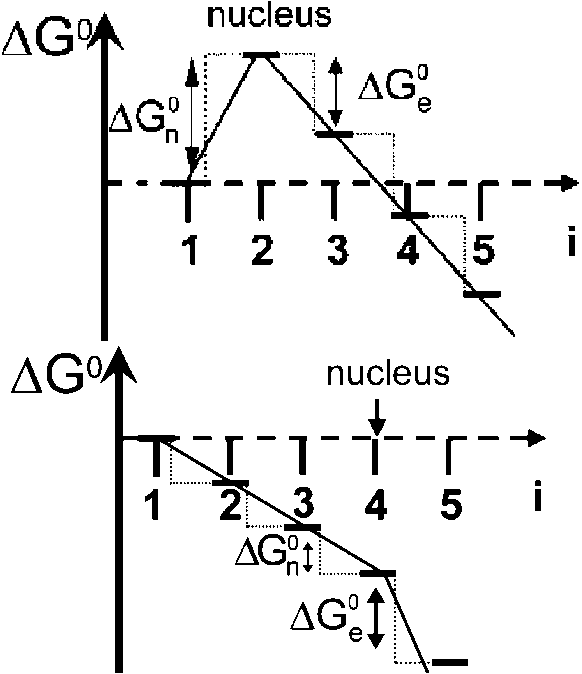
\includegraphics[width=0.9\textwidth]{sec0/cooperativa-2.png}}}\end{figure}
\end{columns}
 \begin{columns}
\column{0.35\linewidth}\begin{figure}{\centering{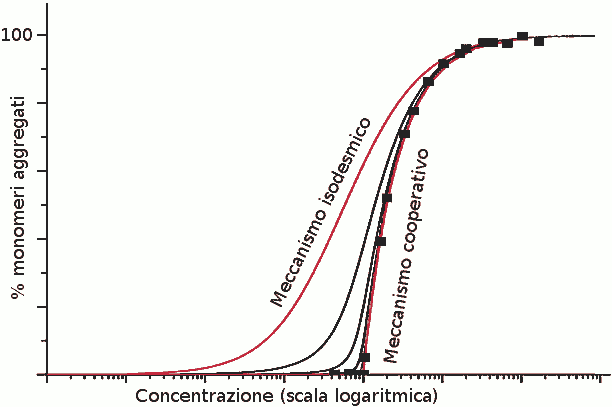
\includegraphics[width=1\textwidth]{sec0/conc.png}}}\end{figure}\column{0.65\linewidth}\begin{figure}{\centering{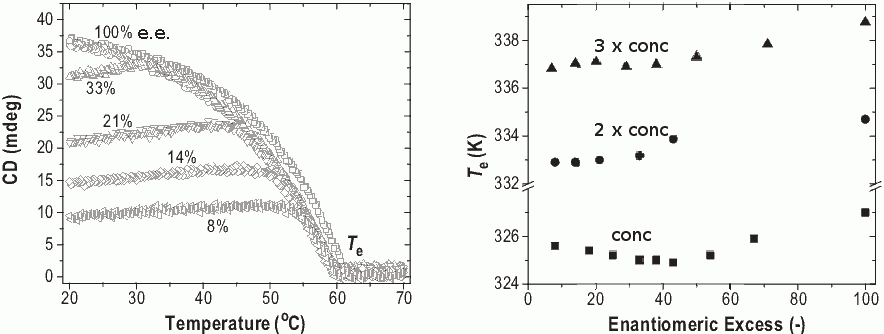
\includegraphics[width=1\textwidth]{sec0/temp_ee.png}}}\end{figure}
\end{columns}
\end{frame}\logo{
\includegraphics[width=0.07\paperwidth]{snslogo.png}}
